\section{University of Hawai'i Cluster}

\subsection{{\craycs}}
\begin{frame}
\frametitle{{\craycs} -- History}
\begin{itemize}
\item[] 2014
  \begin{itemize}
  \item Jul. -- University of {\hawaii} (UH) selects Cray's proposal
  \item Oct. -- Delivered 184 nodes, 3,800 cores
  \item Dec. -- Passed testing and accepted
  \end{itemize}

\item[] 2015
  \begin{itemize}
  \item Jan. -- Early adopter testing started (8 users)
  \item Apr. -- Opened for general use
  \end{itemize}
\item[] 2016
  \begin{itemize}
  \item Mar. -- 92 nodes added, 5,876 cores total
  \end{itemize}
\item[] 2017
  \begin{itemize}
  \item Jan. -- 5 nodes added, 5,992 cores total
  \item Jan. -- 370$+$ users have been granted access to the cluster
  \end{itemize}
\end{itemize}
\end{frame}


\subsubsection{Hardware}
\begin{frame}
  \frametitle{{\craycs} -- Compute Nodes}
  \begin{table}
    \centering
    \resizebox{\textwidth}{!}{%
      \begin{tabular}{|l|l|l|l|l|l|l|l|}
        \multicolumn{8}{c}{ {\large {\textbf{ Community Nodes\footnote{\label{node_note}\tiny Nodes are diskless and run CentOS linux}} } } }\\ \hline
        \textbf{Type} & \textbf{Cores} & \textbf{Ivy-Bridge} & \textbf{Haswell} & \textbf{Broadwell} &
        \textbf{128 GB}\footnote{\label{mem_limit}\tiny Usable RAM: $\approx118$ GB of 128 GB, $\approx246$ GB of 256 GB, $\approx1003$ GB of 1 TB} & \textbf{256 GB}\textsuperscript{\ref{mem_limit}}  & \textbf{1 TB}\textsuperscript{\ref{mem_limit}}  \\ \hline
        Standard & 20 & 178 &  &  & 178 &  &  \\ \hline
        Large & 40 & 6 &  &  &  &  & 6 \\ \hline
        GPU\footnote{\label{gpu_v1}\tiny 2 x Nvidia Tesla K40} & 20 &  & 1 &  & 1 &  & \\ \hline
      \end{tabular}%
    }
  \end{table}

  \begin{table}
    \centering
    \resizebox{\textwidth}{!}{%
      \begin{tabular}{|l|l|l|l|l|l|l|l|}
        \multicolumn{8}{c}{ {\large {\textbf{ Condo Nodes}\textsuperscript{\ref{node_note}} } }} \\ \hline
        \textbf{Type} & \textbf{Cores} & \textbf{Ivy-Bridge} & \textbf{Haswell} & \textbf{Broadwell} & \textbf{128 GB}\textsuperscript{\ref{mem_limit}} & \textbf{256 GB}\textsuperscript{\ref{mem_limit}} & \textbf{1 TB}\textsuperscript{\ref{mem_limit}} \\ \hline
        Standard & 24 & & 62 & & 62 & & \\ \hline
        Standard & 20 & & & (5)\footnote{\label{future}\tiny April 2017 additions} & (5)\textsuperscript{\ref{future}} & & \\ \hline
        Custom & 20 &  & 33 & (4)\textsuperscript{\ref{future}} &  & 33 & (4)\textsuperscript{\ref{future}} \\ \hline
        GPU\textsuperscript{\ref{gpu_v1}}     & 20 &  & 1 &  & 1 &  &  \\ \hline
      \end{tabular}%
    }
    \end{table}
  \end{frame}


\begin{frame}
	\frametitle{{\craycs} -- Storage}
	Two storage options are currently available on the {\craycs}
	\begin{enumerate}
		\item {\lustre}
                  \begin{itemize}
                  \item High performance parallel filesystem 
                  \item Available on all the cluster nodes
                    \item Freely available to all users
                  \end{itemize}
		\item ValueStorage
                  \begin{itemize}
                  \item Network attached scale out storage
                  \item Only available from the login nodes
                  \item Available as a for fee service
                  \end{itemize}
	\end{enumerate}
\end{frame}


\begin{frame}
	\frametitle{{\craycs} -- Storage $\rightarrow$ {\lustre}}
	\begin{itemize}
		\item The {\craycs} has $\approx582$TB of storage space

		\item Primarily used as scratch space for jobs (Input and Output)
		\item User do not have a usage quota (soft or hard)
		\item Certain directories are subject to a 90 day purge policy
		\item \textbf{Data is not backed up!  Users are responsible for their own data}
                \item {\lustre} utilizes RAID 6 arrays, and is fairly robust but \ldots~\\RAID is not a backup
	\end{itemize}
\end{frame}


\begin{frame}
	\frametitle{{\craycs} -- Storage $\rightarrow$ ValueStorage}
        ~\\
	\begin{itemize}
		\item $500$TB of scale out storage
		\item Purchased annually in 0.5TB increments 
	\end{itemize}
	\btVFill

	\begin{center}
	\textbf{ValueStorage Pricing}~\\ 
		\resizebox{0.50\textwidth}{!}{%
		\begin{tabular}{l r }
			\toprule
			\textbf{Product} & \textbf{Annual Cost}~~ \\
	                \midrule
			\midrule
			0.5TB & \$65.00\\
                        0.5TB + Replication  & \$130.00 \\
			\bottomrule
		\end{tabular}
		}
		~\\ \href{http://www.hawaii.edu/its/value-storage-pricing/}{More Information}
		~\\	{\footnotesize \emph{All prices are subject to change}}
	\end{center}
\end{frame}


\begin{frame}
	\frametitle{{\craycs} -- Network}
	\begin{itemize}
		\item 40Gb Infiniband inter-connects (QDR)
		\begin{itemize}
			\item High speed inter-connect between~\\compute nodes, {\lustre} storage and Login nodes
                        \item low latency ($\approx1.3\mu$s)
			\item Utilizes the \emph{fat tree network topology}
			\item[] 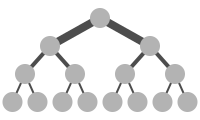
\includegraphics[width=0.20\textwidth]{images/Fat_tree_network} \\[-1ex] {\fontsize{3}{4} \selectfont Source: \url{https://en.wikipedia.org/wiki/Fat_tree} } 		
		\end{itemize}
		\item 10Gb login node internet connectivity
		\begin{itemize}
			\item Speed test from UH to CERN clocked transfer speeds up to 2$+$ Gb/s
		\end{itemize}	
	\end{itemize}
\end{frame}

\subsubsection{Layout}
\begin{frame}
	\frametitle{{\craycs} -- Layout}
	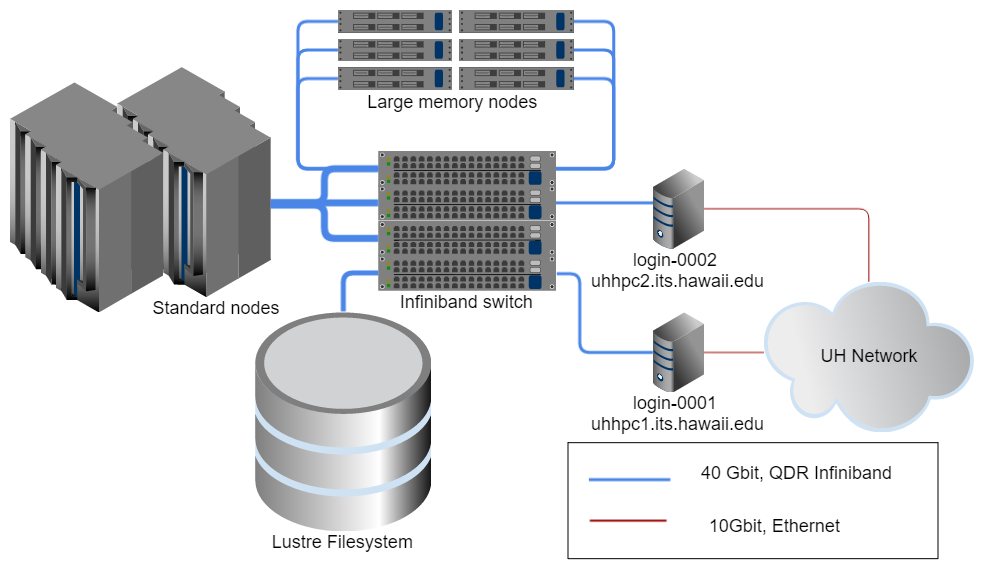
\includegraphics[width=1\textwidth]{images/layout}
\end{frame}

